\section{Results}

We consider a globally isothermal disk, $c_s=\mathrm{const.}$, by
setting $q=0$ in the equation of state, Eq. \ref{eos}, and a flat mid-plane 
gas density, $\rhog(0) = \mathrm{const.}$, so there is no global
radial pressure gradient at the disk midplane. The stopping time is
prescribed as 
\begin{align}
  \tstop = t_\mathrm{s0}\frac{\rho(z=0)}{\rho(z)}. 
\end{align}

As an example, we set the dust-to-gas ratio $\tepsilon_0=0.025$, dust 
scale height $H_\mathrm{d}=0.4\Hgas$, and stopping time
$t_\mathrm{s0}=0.02$. We consider modes with radial wavenumber
$k_x\Hdust=2\pi$. The vertical domain size is set to 
$\zmax=2\Hgas$ and we use $N=513$ grid points. Fig. \ref{eigen_map}
shows a map of the eigenvalues in the $(\omega, s)$ plane. 

\begin{figure}
  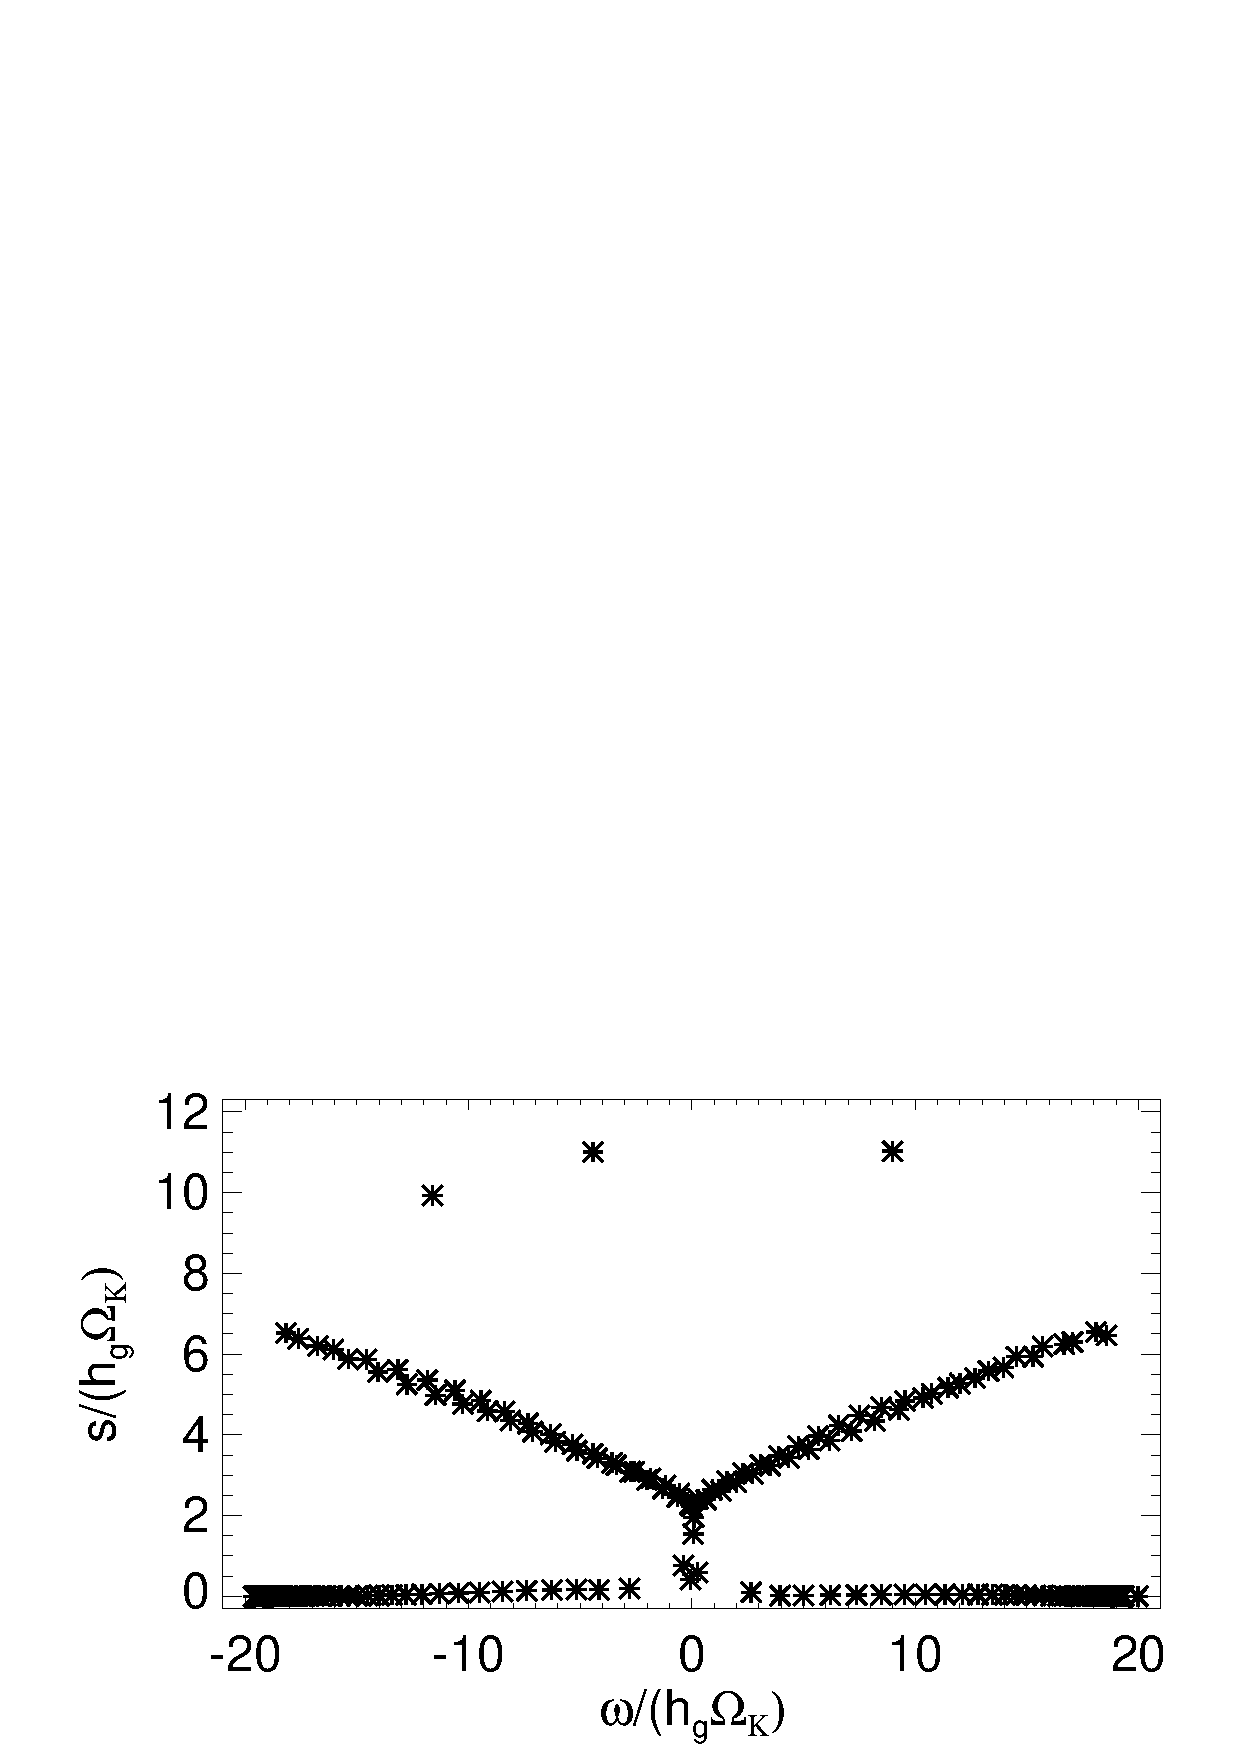
\includegraphics[width=\linewidth]{figures/eigenvalues}
  \caption{Eigenvalues found for the fiducial isothermal dusty
    problem.
  \label{eigen_map}} 
\end{figure}

\begin{figure}
  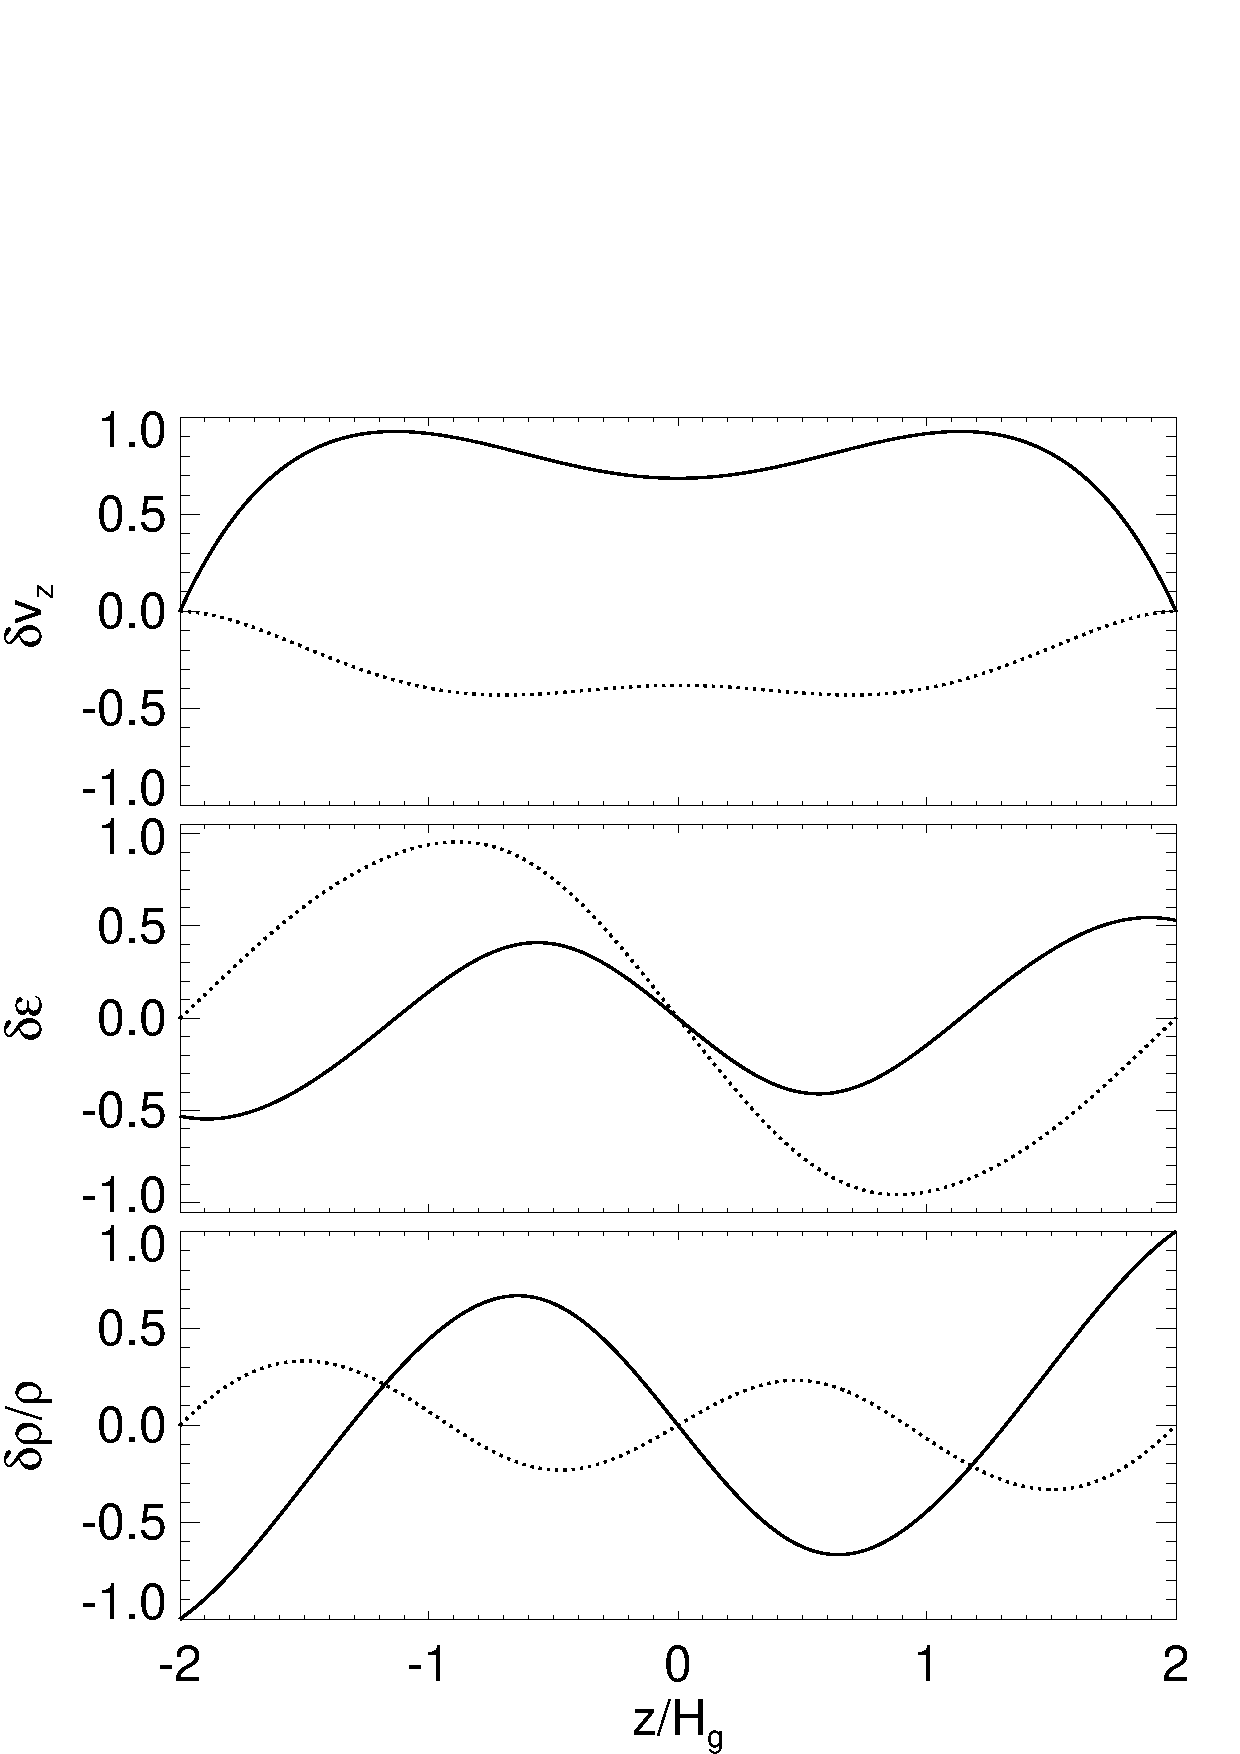
\includegraphics[width=\linewidth]{figures/eigenvec}
  \caption{Example eigenvectors from the fiducial case. 
  \label{eigen_vec}} 
\end{figure}
